\newpage\pagestyle{main}

\chapter{Background e Architettura Generale}\label{chap:first}

\inlineminitoc

% ─────────────────────────────────────────────────────────────────────────────
\section{Stato dell'arte e Motivazioni}

Negli utlimi anni l'avvento dei Large Language Models (LLM) ha segnato un punto di svolta nel campo dell'Intelligenza Artificiale, permettendo interazioni uomo-macchina sempre più naturali e sofisticate \cite{dubey2024llama3}. Questi modelli, addestrati su una quantità enorme di dati testuali, hanno raggiunto capacità notevoli di comprensione e generazione del linguaggio naturale, rivoluzionando il modo in cui le macchine possono assistere gli esseri umani in una vasta gamma di compiti. Tuttavia, nonostante le straordinarie performance, i modelli linguistici pre-addestrati presentano limitazioni intrinseche che ne condizionano l'affidabilità in contesti professionali e scientifici.

% ─────────────────────────────────────────────────────────────────────────────
\subsection{Limiti dei Modelli Linguistici Tradizionali}

Uno segli ostacoli principali è rappresentato dal fenomeno del \textbf{knowledge cutoff}. Un LLM possiede informazioni aggiornate solo fino al momento in cui si è concluso il suo addestramento, quindi se viene posta una domanda su argomenti successivi al periodo di addestramento, il modello non ha accesso alle informazioni più recenti per poter rispondere in modo accurato. Questo non comporta solo una carenza di informazioni aggiornate, ma aumenta il rischio di fornire risposte errate, soprattutto su domini in rapida evoluzione come quello medico, dove nuove scoperte e linee guida cliniche vengono pubblicate regolarmente.

Un altro problema, è appunto rappresentato dalle \textbf{allucinazioni}, dove il modello può generare una risposta sintatticamente corretta ma fattualmente errata o priva di fondamento. Questo fattore, in casi critici come quello medico, può mettere a rischio la sicurezza dell'utente finale, fornendo indicazioni errate, che possono essere prese per veritiere da un utente non esperto.

Inoltre, una \textbf{finestra di contesto} limitata impedisce ad un modello di tenere traccia di tutto quello che viene detto se una conversazione si protrae per un numero elevato di scambi. Questo porta alla perdita di informazioni che posso risultare cruciali per rispondere in modo coerente e accurato, costringendo l'utente a ripetere informazioni già fornite o generando risposte incoerenti con quanto detto in precedenza.

Questi tre limiti sono conseguenze dirette dell'architettura su cui si basano tutti gli LLM odierni. Per ovviare a questi problemi è necessario adottare un approccio diverso, che preveda l'integrazione di una base di conoscenza esterna e aggiornabile in tempo reale.

% ─────────────────────────────────────────────────────────────────────────────
\subsection{L'Approccio Retrieval-Augmented Generation (RAG)}

Per superare queste criticità, è stato adottato il paradigma del \textit{Retrieval-Augmented Generation} (RAG). L'idea alla base del RAG è quella di separare la capacità linguistica di un LLM dalla sua conoscenza. Questo viene realizzato fornendo al modello una base di conoscenza esterna, che viene interrogata in tempo reale per recuperare le informazioni necessarie a rispondere alle domande dell'utente. In questo modo, tenendo il database costantemente aggiornato, viene eliminato il problema del knowledge cutoff fornendo al modello accesso a dati aggiornati. Questo consente anche di ridurre il rischio di allucinazioni dato che le risposte sono basate su fonti verificabili.

Per attuare il processo RAG, vengono eseguite le seguenti operazioni in sequenza:
\begin{enumerate}
    \item \textbf{Retrieve (Recupero)}: Quando l'utente pone una domanda il sistema esegue una ricerca all'interno della base di conoscenza esterna identificando i documenti più rilevanti per rispondere alla domanda. Questa fase è cruciale per l'accuratezza della risposta.
    \item \textbf{Augment (Arricchimento)}: Una volta recuperati i documenti utili a rispondere alla domanda, questi vengono fortini come promt aggiuntivo al modello linguistico, che in questo modo riesce ad arricchire la sua conoscenza e comprensione del dominio.
    \item \textbf{Generate (Generazione)}: Infine il modello, grazie alla conoscenza ricevuta, è in grado di generare una risposta quanto più accurata possibile. Questa risposta viene poi restituita all'untente, completando il ciclo di interazione.
\end{enumerate}

\newpage

La maggior parte delle implementazioni RAG si basano su database di tipo vettoriale, che permettono di effettuare ricerche per similarità semantica tra le domande dell'utente e i documenti presenti nel database stesso. Nel lavoro svolto in questa tesi si è scelto di adottare un approccio ibrido, integrando la ricerca per similarità vettoriale con una rappresentazione a grafo dei documenti. In questo modo è possibile sfruttare la struttura fornita dal grafo per navigare i documenti stessi. Questo viene utilizzato per recuperare non solo sigole porzioni di testo, ma anche una finestra di contensto più ampia, in modo da ridurre ulteriormente il rischio di allucinazioni e migliorare la coerenza delle risposte generate.

\begin{figure}[htbp]
    \centering
    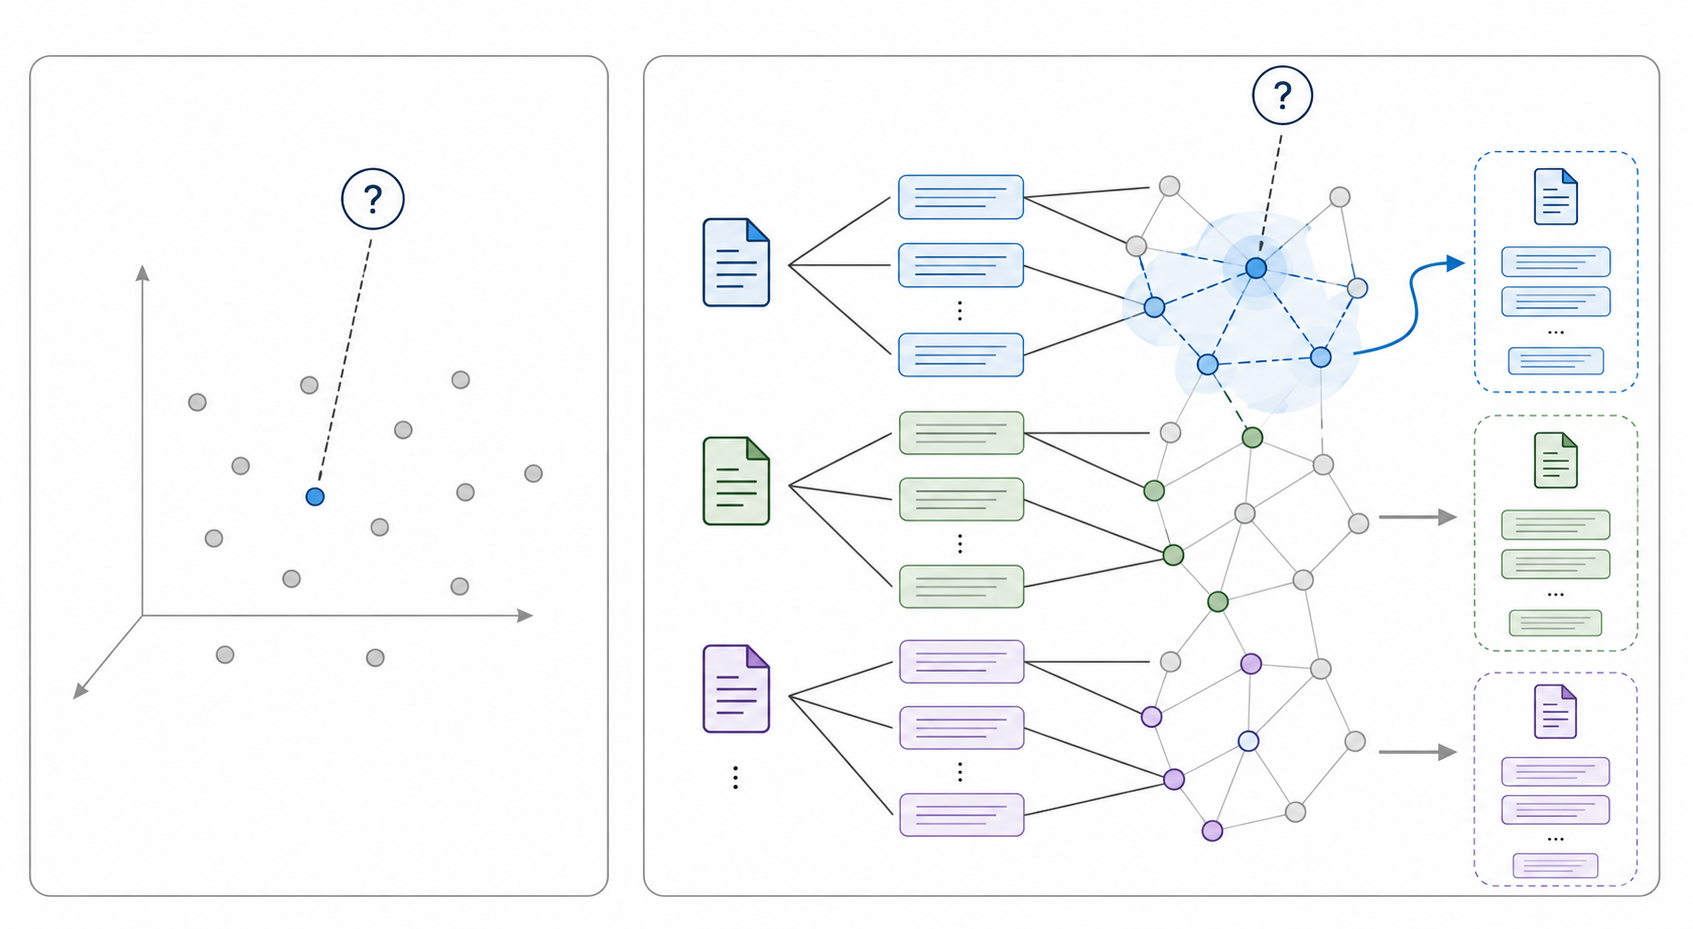
\includegraphics[width=1\textwidth]{_figures/rag_vs_graphrag.png}
    \caption{Confronto concettuale tra un sistema vettoriale ed un sistema ibrido a grafo.}
    \label{fig:rag_vs_graphrag}
\end{figure}

% ─────────────────────────────────────────────────────────────────────────────
\section{Tecnologie Utilizzate}

L'impostazione tecnologica del sistema è stata scelta per garantire un'esecuzione quando più indipendente possibile da servizi esterni, massimizzando performance in termini di latenza e garantendo una sicurezza nella gestione dei dati, i quali non lasciano mai la macchina locale. Di seguito vendono descritte le tecnologie principali utilizzate per lo sviluppo del sistema, con un focus sulle motivazioni che hanno guidato la scelta di ciascuna di esse.

\newpage

% ─────────────────────────────────────────────────────────────────────────────
\subsection{Orchestrazione e Linguaggio}

Il componente principale del sistema, che rappresenta l'unità logica dell'agente conversazionale, è sviluppato in \textbf{Python} \cite{python}, sfruttando il framework \textbf{LangGraph} \cite{langgraph}. La scelta di Python è motivata dall'ampio ecosistema di librerie disponibili per il Machine Learning, la gestione di database e la manipolazione di dati strutturati, che ha permesso di ridurre significativamente i tempi di sviluppo e di integrazione tra i diversi componenti del sistema.

LangGraph in particolare è stato scelto per la sua capacità di modellare flussi di lavoro dinamici, che sono risultati essenziali per la gestione di un Conversational AI basato su RAG. In questo modello ogni nodo del grafo rappresenta un'azione che l'agente può eseguire, e gli archi definiscono le transizioni tra un'azione e la successiva. Questa architettura è risultata fondamentale nello sviluppo del sistema, perché ha permesso di gestire due percorsi di esecuzione distinti. Se la domanda dell'utente è una domanda di conversazione generica, questa può essere gestita direttamente dall'LLM senza accedere al database, eliminando completamente i costi di latenza associati alla ricerca e al recupero dei documenti. Se invece la domanda richiede il recupero di informazioni specifiche, il sistema attiva automaticamente la ricerca dei documenti rilevanti per rispondere alla domanda. Questa flessibilità è stata cruciale per garantire un'esperienza utente fluida e naturale, evitando ritardi inutili per domande che non richiedono accesso alla base di conoscenza.

% ─────────────────────────────────────────────────────────────────────────────
\subsection{Modelli di Intelligenza Artificiale e Hosting Locale}

Il sistema si basa su modelli di intelligenza artificiale eseguiti in locale tramite \textbf{Ollama} \cite{ollama}. Questa scelta è stata dettata sia da considerazioni di sicurezza e privacy, dato che il dominio dei dati è quello medico, sia per abbattere i costi di utilizzo di servizi cloud in termini di costi economici e latenza. I modelli utilizzati per le operazioni di ragionamento ed embedding sono i seguenti:

\begin{itemize}
    \item \textbf{Llama 3.2 (3b)} \cite{dubey2024llama3}: Utilizzato come modello di base per il ragionamento e la generazione del testo. La versione del modello con 3 miliardi di parametri è stata scelta, a confronto con versioni più grandi, per garantire un equilibrio ottimale tra capacità di comprensione e generazione del linguaggio naturale e requisiti computazionali, permettendo un'esecuzione che no comprometta la qualità del servizio senza necessitare di risorse eccessive.

    \item \textbf{Embedding-Gemma} \cite{embedding_gemma_2025}: Utilizzato per la generazione di embedding vettoriali, fondamentali per la ricerca per similarità all'interno del database. Embedding-Gemma è stato scelto per la sua capacità di produrre rappresentazioni semantiche di alta qualità, che migliorano significativamente l'accuratezza della ricerca e del recupero dei documenti rilevanti.
\end{itemize}

% ─────────────────────────────────────────────────────────────────────────────
\subsection{Data Management e Interfaccia}

La gestione dei dati per la base di conoscenza è affidata a \textbf{Neo4j} \cite{neo4j}, un DBMS a grafo che si adatta perfettamente alla rappresentazione strutturata dei documenti utilizzati in questo progetto. Neo4j permette di modellare i documenti come nodi e le relazioni tra essi e le loro porzioni di testo come archi, facilitando la navigazione e il recupero di informazioni. Inoltre, Neo4j supporta nativamente la ricerca per similarità vettoriale, il che ha permesso un'integrazione fluida con il modello di embedding, senza dover ricorrere a soluzioni di terze parti per la gestione dei vettori.

L'interfaccia utente è stata realizzata in \textbf{Unreal Engine} \cite{ue} attraverso il plugin \textbf{FANTASIA} \cite{fantasia1, fantasia2}. FANTASIA è un plugin che consente la creazione facilitata di agenti virtuali intelligenti, fornendo un'integrazione nativa con modelli di intelligenza artificiale e strumenti di orchestrazione come LangGraph. L'utilizzo di Unreal Engine ha permesso di creare un ambiente immersivo e interattivo, in cui l'agente virtuale può rispondere alle domande dell'utente in modo naturale, con supporto per la sintesi vocale e il lip sync, migliorando significativamente l'esperienza utente.

% ─────────────────────────────────────────────────────────────────────────────
\section{Architettura Distribuita e Logica di Sharding}

In scenare reali, applicazioni di conversational AI basate su RAG possono dover gestire basi di conoscenza di dimensioni molto maggiori, con milioni di nodi e relazioni. In questi casi, l'accesso a un database remoto può introdurre una latenza significativa, che si somma a quella del modello di intelligenza artificiale e degli altri componenti del sistema, come la sintesi vocale o il lip sync utilizzato per la maggiore immersività dell'agente virtuale, compromettendo la fluidità dell'interazione \cite{latency_eca} e rendendo vano il vantaggio dell'uso di modelli di intelligenza artificiale.

Per affrontare questo problema, il sistema adotta un'architettura ispirata ai principi del \textit{data sharding} e del \textit{caching} applicati ai database distribuiti \cite{kleppmann2017}. Si noti che, nel corso di una conversazione, l'agente tende ad accedere ripetutamente a un sottoinsieme ristretto dei documenti messi a disposizione. Quindi questo sottoinsieme può essere tenuto in memoria locale per minimizzare il passaggio di dati dal database remoto, riducendo così i costi di latenza e migliorando le performance complessive del sistema. Il database locale funge a tutti gli effetti da cache intelligente, che si aggiorna dinamicamente in base alle esigenze della conversazione e alla frequenza di accesso ai documenti.

\newpage

% ─────────────────────────────────────────────────────────────────────────────
\subsection{Modello a Due Livelli: Remote vs Shard}

Il sistema è quindi strutturato su due livelli distinti per la gestione dei dati:

\begin{enumerate}
    \item \textbf{Remote Storage}: Risiede su un server Neo4j dedicato e contiene l'intera base di conoscenza. Nel caso specifico di questo progetto è stato utilizzato il servizio \textit{Neo4j Aura} per ospitare il database in cloud. Il Remote è il database che viene interrogato per la ricerca iniziale o per recuperare documenti che non sono ancora stati sincronizzati nello Shard locale.

    \item \textbf{Local Shard}: Risiede sulla macchina locale e contiene solo un sottoinsieme dei documenti più rilevanti per la conversazione in corso. Lo Shard funge da cache ad alta velocità, che viene popolata dinamicamente con i documenti recuperati dal Remote. Le query successive alla prima, a meno di cache-miss, resituiscono risultati direttamente dallo Shard, riducendo drasticamente la latenza percepita dall'utente.
\end{enumerate}

Questa separazione trasforma il problema del recupero dati in una strategia di \textbf{caching intelligente}. Quando il sistema recupera informazioni dal Remote, queste vengono sincronizzate nello Shard locale, avvicinando così i dati all'utente. Le interrogazioni successive avverranno direttamente sulla memoria locale, riducendo drasticamente la latenza percepita dall'utente. L'implementazione di questa logica necessita di una gestione del contenuto dello Shard, questo per evitare l'appesantimento dello stesso, che porterebbe inevitabilmente ad un degrado delle performance. Per questo motivo, ad ogni accesso al Remote, il sistema aggiorna dei metadati di utilizzo che alimentano la politica di eviction, garantendo che lo Shard rimanga snello ed efficiente anche nel corso di sessioni prolungate.

\begin{figure}[htbp]
    \centering
    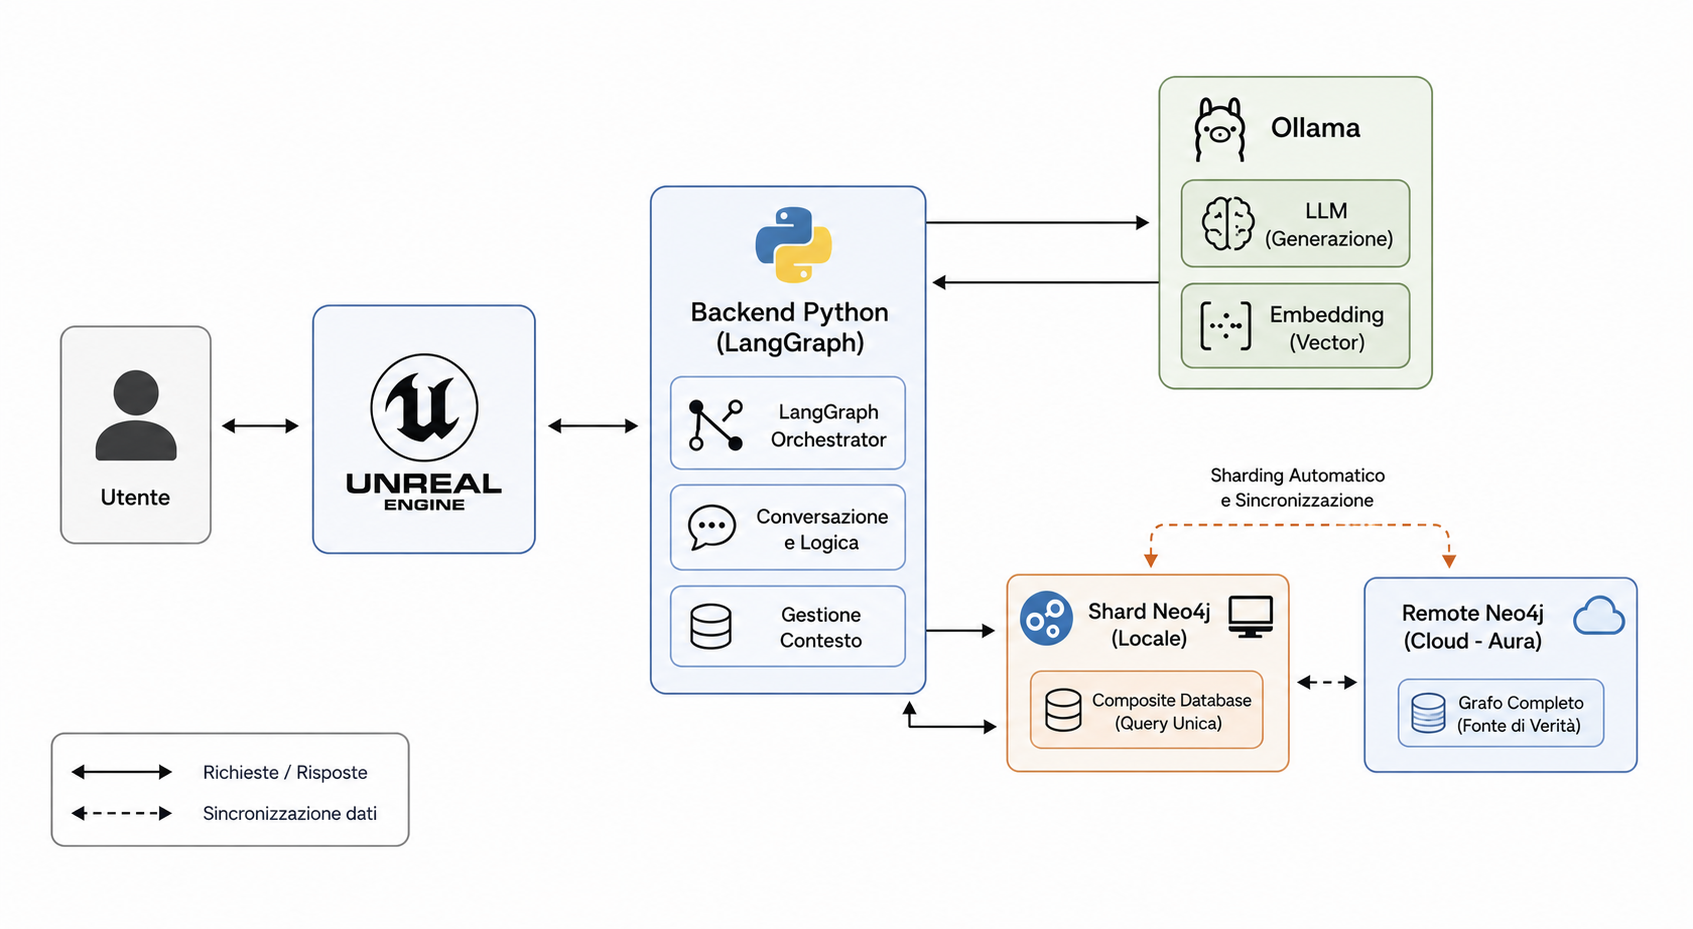
\includegraphics[width=1\textwidth]{_figures/system_architecture.png}
    \caption{Architettura ad alto livello del sistema distribuito.}
    \label{fig:architettura}
\end{figure}

\newpage

% ─────────────────────────────────────────────────────────────────────────────
\section{Ottimizzazione delle Query e Execution Plan Cache}

Un'ulteriore ottimizzazione è stata implementata a livello di query Cypher, per massimizzare le performance del database Neo4j. In un sistema RAG distribuito, la latenza delle query al database è un fattore critico che può influenzare significativamente l'esperienza utente. Per questo motivo, è stato adottato un approccio sistematico all'ottimizzazione delle query, con particolare attenzione alla gestione dell'Execution Plan Cache di Neo4j.

La soluzione è stata quella di parametrizzare le query Cypher, in modo da massimizzare il riutilizzo dei piani di esecuzione. In questo modo, quando una query viene eseguita per la prima volta, Neo4j compila un piano di esecuzione ottimizzato per quella specifica query. Essendo che il sistema è stato strutturato per eseguire tutte le operazioni di sincronizzazione e manutenzione dello Shard locale all'interno della stessa query Cypher, è possibile garantire che lo stesso piano di esecuzione venga riutilizzato costantemente durante la conversazione, riducendo così i tempi di esecuzione delle query successive.

Il beneficio di questa ottimizzazione è doppio, in quanto non solo riduce la latenza delle query al database, ma contribuisce anche a stabilizzare le performance del sistema, evitando picchi di latenza dovuti alla compilazione di nuovi piani di esecuzione per ogni query. Questo è particolarmente importante in un contesto di Conversational AI, dove la reattività del sistema è fondamentale per garantire un'esperienza utente fluida e naturale.

% ─────────────────────────────────────────────────────────────────────────────

\section{Workflow del Sistema}

Il workflow completo del sistema, che integra tutte le componenti descritte nei paragrafi precedenti, può essere sintetizzato nei seguenti passaggi:

\begin{enumerate}
    \item \textbf{Input e Trascrizione}: L'audio dell'utente viene catturato dall'agente virtuale in Unreal Engine e trascritto in testo tramite il modulo \textbf{Whisper ASR} \cite{whisper}, fornito da FANTASIA. La trascrizione viene quindi inviata al server LangGraph.

    \item \textbf{Decisione contestuale}: Il server LangGraph analizza il messaggio dell'utente e determina tramite LLM se si tratta di una domanda di conversazione generica o di una domanda che richiede il recupero di informazioni specifiche. Se è una domanda generica, viene inviata direttamente al modello Llama 3.2 per la generazione della risposta, bypassando completamente il database. Se invece è una domanda che richiede il recupero di informazioni, si attiva la logica di sharding descritta nei passaggi successivi.

    \item \textbf{Ricerca e Sincronizzazione}: Il sistema genera l'embedding del messaggio dell'utente e lo utilizza per eseguire una ricerca per similarità all'interno del Remote Storage. I paragrafi dei documenti più rilevanti vengono recuperati e sincronizzati nello Shard locale insieme ad un contesto di $\pm 2$ paragrafi.

          \newpage

    \item \textbf{Manutenzione (Eviction)}: Ad ogni sincronizzazione, i metadati di utilizzo dei documenti nello Shard vengono aggiornati. Se lo Shard supera una soglia predefinita di capacità, viene attivata la politica di eviction basata su LFU (Least Frequently Used), che rimuove i documenti meno utilizzati per fare spazio a quelli più rilevanti per la conversazione in corso.

    \item \textbf{Generazione e Risposta}: Il modello Llama 3.2 genera una risposta basata sui documenti presenti nello Shard locale, che viene poi restituita a Unreal Engine, il quale tramite il modulo di sintesi vocale \textbf{ElevenLabs} \cite{elevenlabs} genera l'audio risultante che sarà riprodotto dall'agente virtuale.
\end{enumerate}

\begin{figure}[htbp]
    \centering
    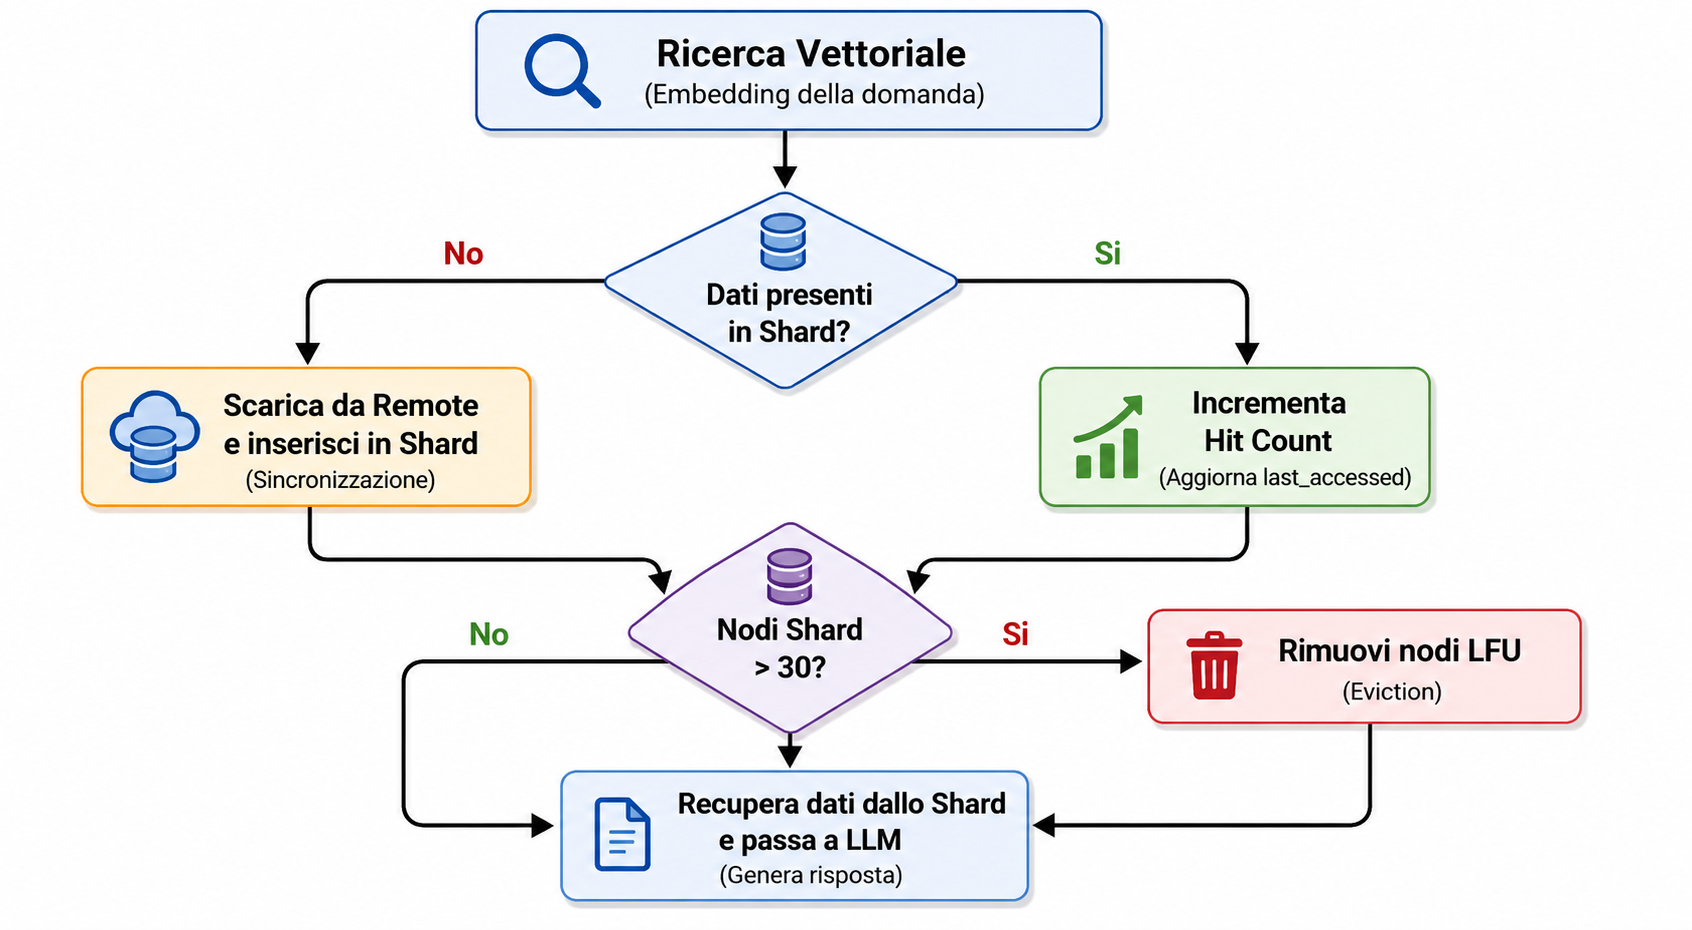
\includegraphics[width=1\textwidth]{_figures/sharding_flowchart.png}
    \caption{Diagramma di flusso della logica di sincronizzazione e manutenzione dello Shard locale.}
    \label{fig:flowchart}
\end{figure}

\begin{figure}[htbp]
    \centering
    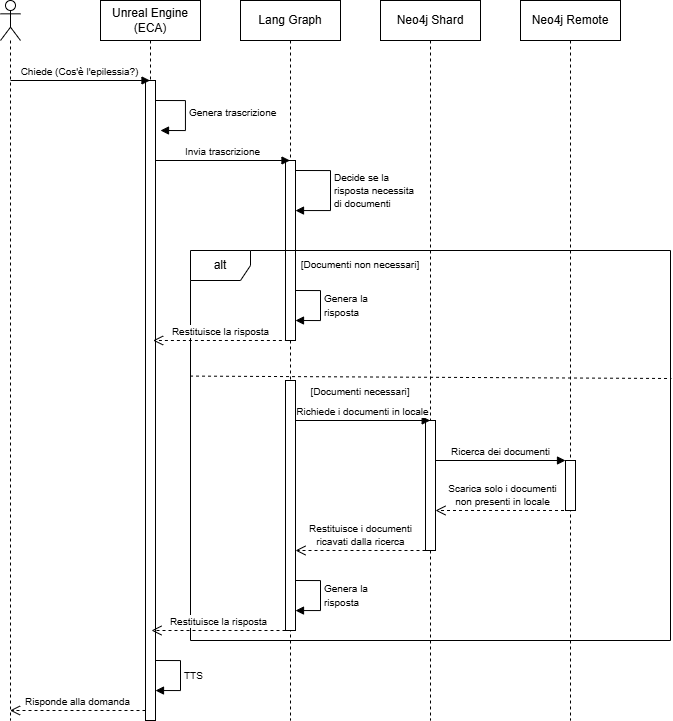
\includegraphics[width=1\textwidth]{_figures/sequence_diagram.png}
    \caption{Sequence diagram dell'interazione completa.}
    \label{fig:sequence}
\end{figure}